\documentclass{standalone}
\usepackage{tikz}
\usepackage{ctex,siunitx}
\usepackage{tkz-euclide}
\usepackage{amsmath}
\usetikzlibrary{patterns, calc}
\usetikzlibrary {decorations.pathmorphing, decorations.pathreplacing, decorations.shapes,}
\begin{document}
\small
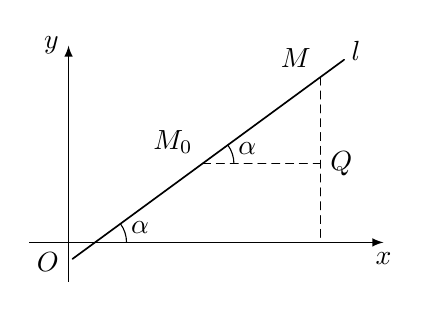
\begin{tikzpicture}[>=latex,scale=1.0]
  \tkzDefPoints{0/0/O,1/0/x,0/1/y,1.7/1/M0,3.2/2.1/M}
  \tkzDefPointsBy[projection=onto O--x](M){P}
  \tkzDefPointsBy[projection=onto M--P](M0){Q}
  \tkzInterLL(M,M0)(O,x)\tkzGetPoint{A}
  \draw[thin,->](-0.5,0)--(4,0)node[below]{$x$};
  \draw[thin,->](0,-0.5)--(0,2.5)node[left]{$y$};
  \tkzDrawLine[semithick,add=1.1 and 0.2](M0,M)
  \tkzLabelLine[pos=1.3](M0,M){$l$}
  \tkzDrawSegments[densely dashed](M,P M0,Q)
  \tkzMarkAngle[size=0.4](x,A,M)
  \tkzLabelAngle[pos=0.6](x,A,M){$\alpha$}
  \tkzMarkAngle[size=0.4](Q,M0,M)
  \tkzLabelAngle[pos=0.6](Q,M0,M){$\alpha$}
  \tkzLabelPoints[below left](O)
  \tkzLabelPoints[right](Q)
  \tkzLabelPoints[above left](M)
  \tkzLabelPoint[above left](M0){$M_0$}
\end{tikzpicture}
\end{document}